% Architecture Diagrams for AML-RL Framework
% Compile standalone or include in main document

\documentclass[tikz,border=10pt]{standalone}

\usepackage{tikz}
\usetikzlibrary{shapes,arrows,positioning,fit,backgrounds,calc}

\begin{document}

% ============================================================================
% DIAGRAM 1: Full System Architecture
% ============================================================================
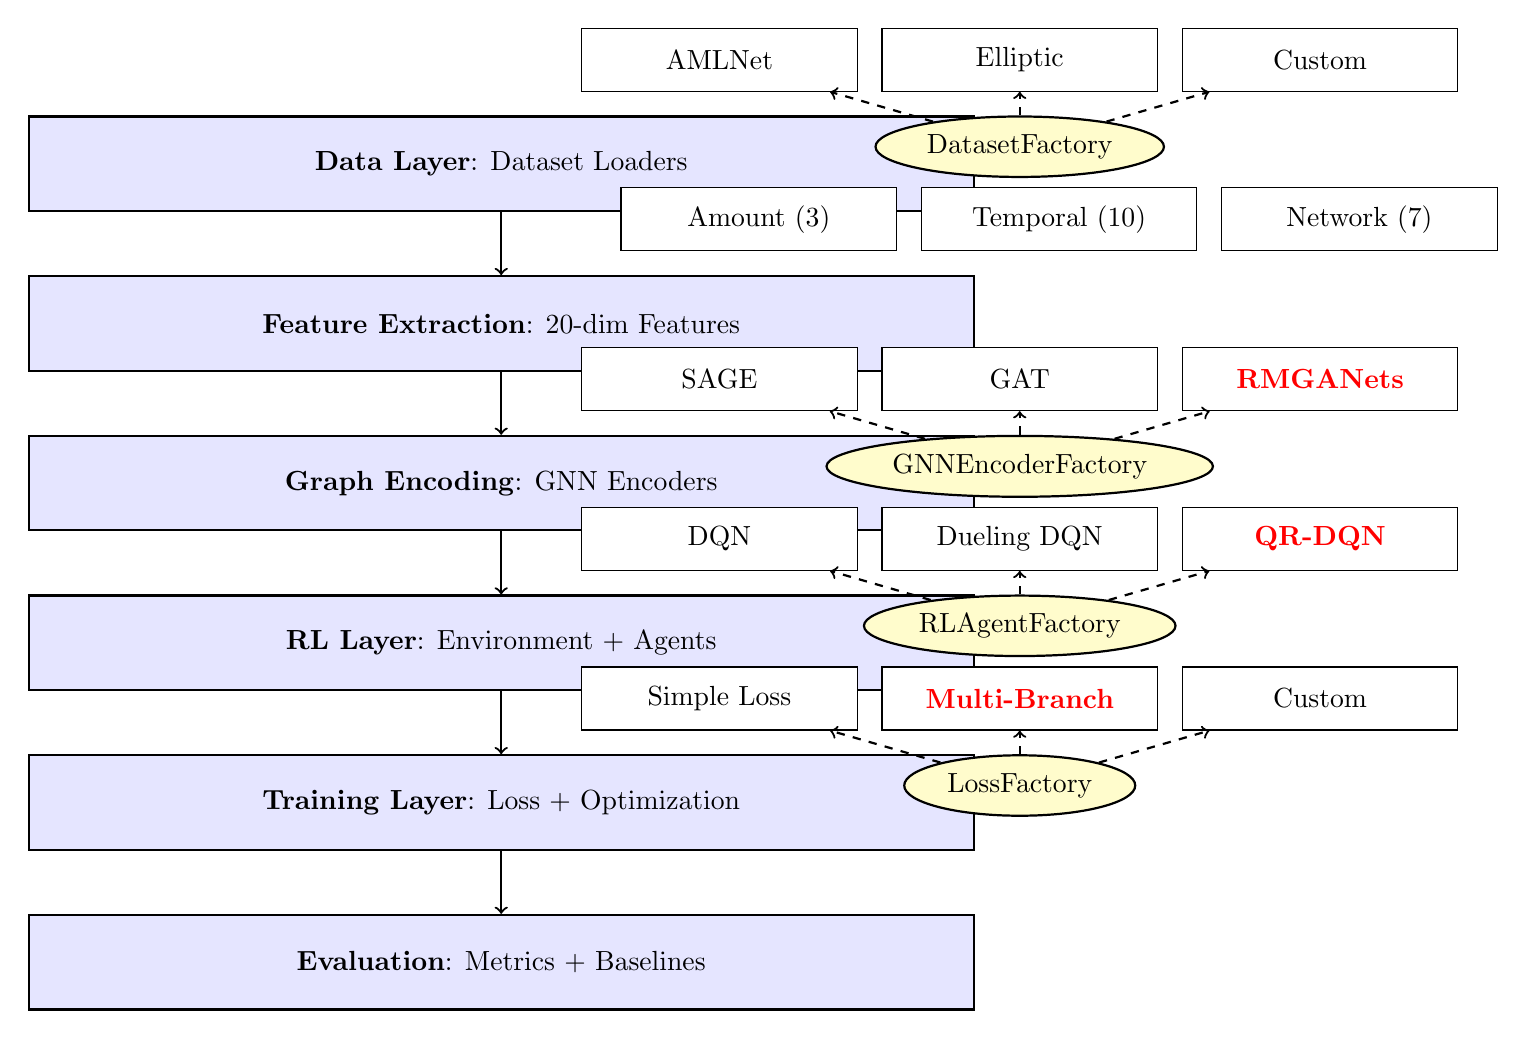
\begin{tikzpicture}[
    node distance=0.8cm and 1.5cm,
    layer/.style={rectangle, draw, thick, minimum width=12cm, minimum height=1.2cm, align=center, fill=blue!10},
    component/.style={rectangle, draw, minimum width=3.5cm, minimum height=0.8cm, align=center, fill=white},
    factory/.style={ellipse, draw, thick, minimum width=2.5cm, fill=yellow!20},
    arrow/.style={->, thick},
    label/.style={font=\small\bfseries}
]

    % Layers
    \node[layer] (data) {\textbf{Data Layer}: Dataset Loaders};
    \node[layer, below=of data] (features) {\textbf{Feature Extraction}: 20-dim Features};
    \node[layer, below=of features] (gnn) {\textbf{Graph Encoding}: GNN Encoders};
    \node[layer, below=of gnn] (rl) {\textbf{RL Layer}: Environment + Agents};
    \node[layer, below=of rl] (train) {\textbf{Training Layer}: Loss + Optimization};
    \node[layer, below=of train] (eval) {\textbf{Evaluation}: Metrics + Baselines};

    % Components in Data Layer
    \node[component, above right=0.3cm and -5cm of data] (amlnet) {AMLNet};
    \node[component, right=0.3cm of amlnet] (elliptic) {Elliptic};
    \node[component, right=0.3cm of elliptic] (custom) {Custom};
    \node[factory, below=0.3cm of elliptic] (datafactory) {DatasetFactory};

    % Components in Feature Layer
    \node[component, above right=0.3cm and -4.5cm of features] (amount) {Amount (3)};
    \node[component, right=0.3cm of amount] (temporal) {Temporal (10)};
    \node[component, right=0.3cm of temporal] (network) {Network (7)};

    % Components in GNN Layer
    \node[component, above right=0.3cm and -5cm of gnn] (sage) {SAGE};
    \node[component, right=0.3cm of sage] (gat) {GAT};
    \node[component, right=0.3cm of gat] (rmganets) {\color{red}\textbf{RMGANets}};
    \node[factory, below=0.3cm of gat] (gnnfactory) {GNNEncoderFactory};

    % Components in RL Layer
    \node[component, above right=0.3cm and -5cm of rl] (dqn) {DQN};
    \node[component, right=0.3cm of dqn] (dueling) {Dueling DQN};
    \node[component, right=0.3cm of dueling] (qrdqn) {\color{red}\textbf{QR-DQN}};
    \node[factory, below=0.3cm of dueling] (agentfactory) {RLAgentFactory};

    % Components in Training Layer
    \node[component, above right=0.3cm and -5cm of train] (simpleloss) {Simple Loss};
    \node[component, right=0.3cm of simpleloss] (multibranch) {\color{red}\textbf{Multi-Branch}};
    \node[component, right=0.3cm of multibranch] (customloss) {Custom};
    \node[factory, below=0.3cm of multibranch] (lossfactory) {LossFactory};

    % Arrows between layers
    \draw[arrow] (data) -- (features);
    \draw[arrow] (features) -- (gnn);
    \draw[arrow] (gnn) -- (rl);
    \draw[arrow] (rl) -- (train);
    \draw[arrow] (train) -- (eval);

    % Factory connections
    \draw[arrow, dashed] (datafactory) -- (amlnet);
    \draw[arrow, dashed] (datafactory) -- (elliptic);
    \draw[arrow, dashed] (datafactory) -- (custom);
    \draw[arrow, dashed] (gnnfactory) -- (sage);
    \draw[arrow, dashed] (gnnfactory) -- (gat);
    \draw[arrow, dashed] (gnnfactory) -- (rmganets);
    \draw[arrow, dashed] (agentfactory) -- (dqn);
    \draw[arrow, dashed] (agentfactory) -- (dueling);
    \draw[arrow, dashed] (agentfactory) -- (qrdqn);
    \draw[arrow, dashed] (lossfactory) -- (simpleloss);
    \draw[arrow, dashed] (lossfactory) -- (multibranch);
    \draw[arrow, dashed] (lossfactory) -- (customloss);

\end{tikzpicture}

\newpage

% ============================================================================
% DIAGRAM 2: RMGANets Module Architecture
% ============================================================================
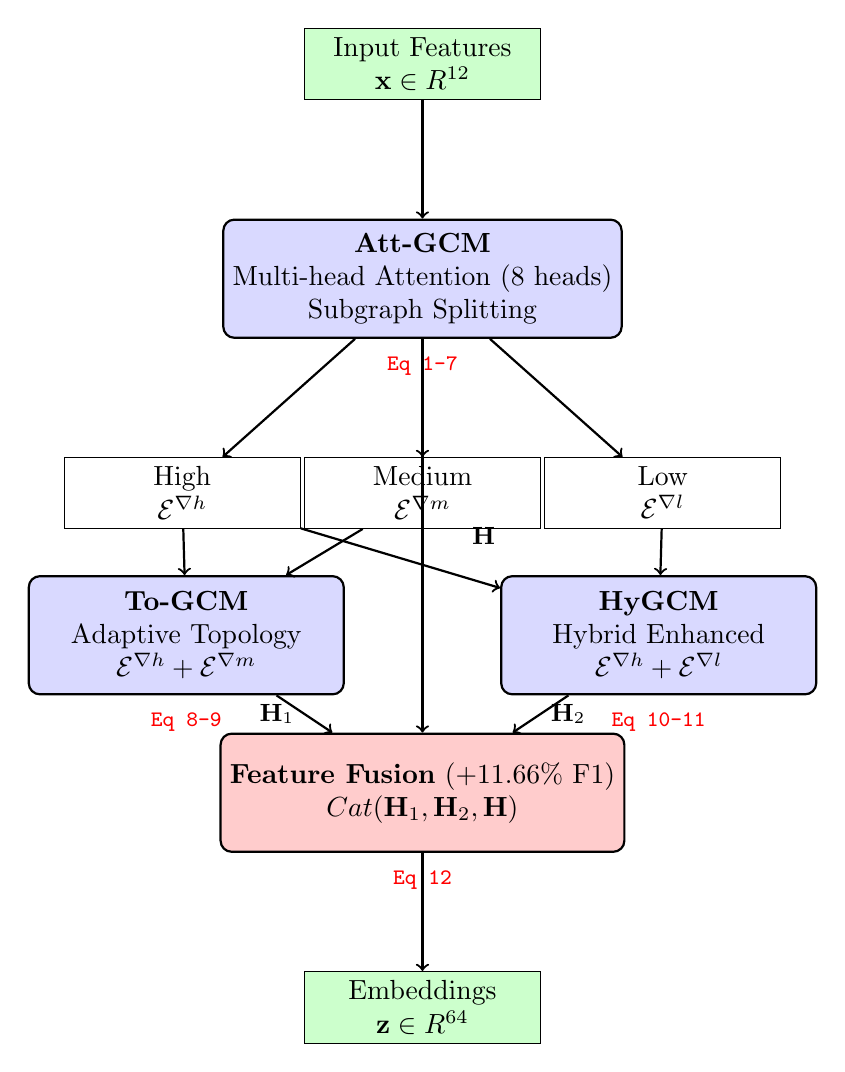
\begin{tikzpicture}[
    node distance=1.5cm,
    module/.style={rectangle, draw, thick, minimum width=4cm, minimum height=1.5cm, align=center, fill=blue!15, rounded corners},
    submodule/.style={rectangle, draw, minimum width=3cm, minimum height=0.8cm, align=center, fill=white},
    arrow/.style={->, thick},
    label/.style={font=\small},
    eq/.style={font=\footnotesize\ttfamily, text=red}
]

    % Input
    \node[submodule, fill=green!20] (input) {Input Features\\$\mathbf{x} \in \mathbb{R}^{12}$};

    % Att-GCM
    \node[module, below=of input] (attgcm) {
        \textbf{Att-GCM}\\
        Multi-head Attention (8 heads)\\
        Subgraph Splitting
    };
    \node[eq, below=0.1cm of attgcm] {Eq 1-7};

    % Split into 3 paths
    \node[submodule, below left=1.5cm and -1cm of attgcm] (high) {High\\$\mathcal{E}^{\nabla h}$};
    \node[submodule, below=1.5cm of attgcm] (medium) {Medium\\$\mathcal{E}^{\nabla m}$};
    \node[submodule, below right=1.5cm and -1cm of attgcm] (low) {Low\\$\mathcal{E}^{\nabla l}$};

    % To-GCM
    \node[module, below=3cm of attgcm, xshift=-3cm] (togcm) {
        \textbf{To-GCM}\\
        Adaptive Topology\\
        $\mathcal{E}^{\nabla h} + \mathcal{E}^{\nabla m}$
    };
    \node[eq, below=0.1cm of togcm] {Eq 8-9};

    % HyGCM
    \node[module, below=3cm of attgcm, xshift=3cm] (hygcm) {
        \textbf{HyGCM}\\
        Hybrid Enhanced\\
        $\mathcal{E}^{\nabla h} + \mathcal{E}^{\nabla l}$
    };
    \node[eq, below=0.1cm of hygcm] {Eq 10-11};

    % Fusion
    \node[module, below=5cm of attgcm, fill=red!20] (fusion) {
        \textbf{Feature Fusion} (+11.66\% F1)\\
        $\text{Cat}(\mathbf{H}_1, \mathbf{H}_2, \mathbf{H})$
    };
    \node[eq, below=0.1cm of fusion] {Eq 12};

    % Output
    \node[submodule, fill=green!20, below=of fusion] (output) {Embeddings\\$\mathbf{z} \in \mathbb{R}^{64}$};

    % Arrows
    \draw[arrow] (input) -- (attgcm);
    \draw[arrow] (attgcm) -- (high);
    \draw[arrow] (attgcm) -- (medium);
    \draw[arrow] (attgcm) -- (low);
    \draw[arrow] (high) -- (togcm);
    \draw[arrow] (medium) -- (togcm);
    \draw[arrow] (high) -- (hygcm);
    \draw[arrow] (low) -- (hygcm);
    \draw[arrow] (togcm) -- node[left, label] {$\mathbf{H}_1$} (fusion);
    \draw[arrow] (hygcm) -- node[right, label] {$\mathbf{H}_2$} (fusion);
    \draw[arrow] (attgcm) -- node[right, label, xshift=0.5cm] {$\mathbf{H}$} (fusion);
    \draw[arrow] (fusion) -- (output);

\end{tikzpicture}

\newpage

% ============================================================================
% DIAGRAM 3: Multi-Branch Loss Components
% ============================================================================
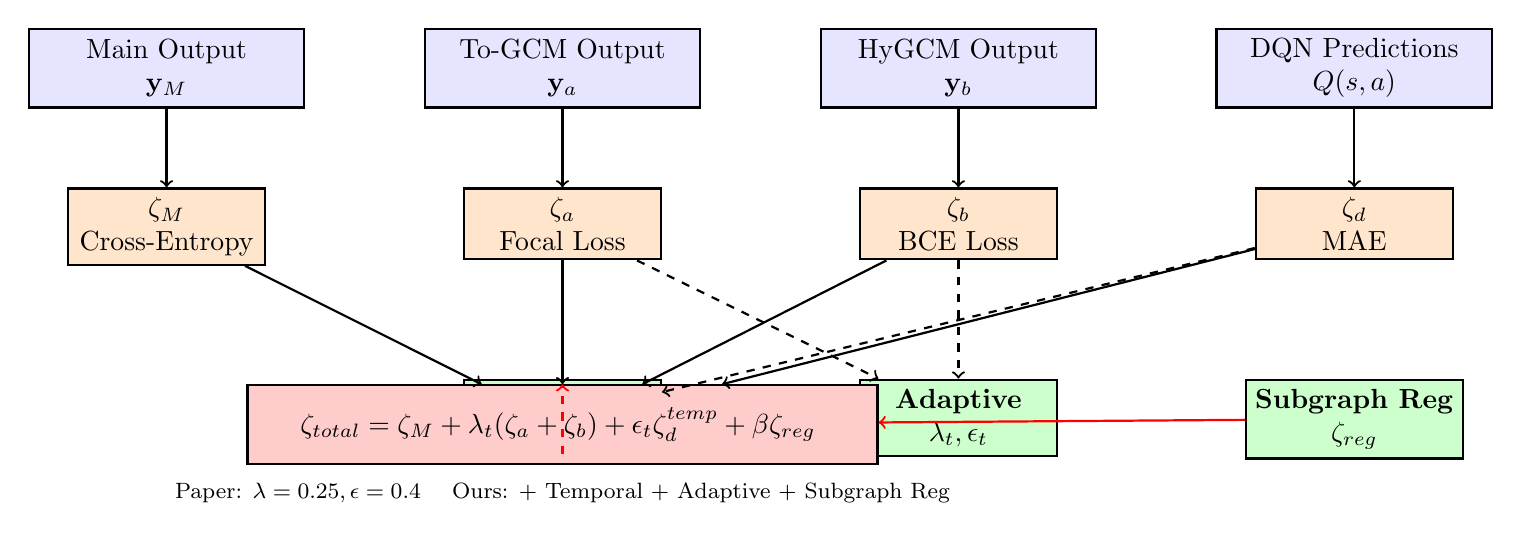
\begin{tikzpicture}[
    node distance=1cm,
    component/.style={rectangle, draw, thick, minimum width=3.5cm, minimum height=1cm, align=center, fill=blue!10},
    loss/.style={rectangle, draw, thick, minimum width=2.5cm, minimum height=0.8cm, align=center, fill=orange!20},
    improvement/.style={rectangle, draw, thick, minimum width=2.5cm, minimum height=0.8cm, align=center, fill=green!20},
    arrow/.style={->, thick},
    label/.style={font=\footnotesize}
]

    % Main components
    \node[component] (main) {Main Output\\$\mathbf{y}_M$};
    \node[component, right=1.5cm of main] (to) {To-GCM Output\\$\mathbf{y}_a$};
    \node[component, right=1.5cm of to] (hy) {HyGCM Output\\$\mathbf{y}_b$};
    \node[component, right=1.5cm of hy] (dqn) {DQN Predictions\\$Q(s,a)$};

    % Loss components
    \node[loss, below=of main] (cemain) {$\zeta_M$\\Cross-Entropy};
    \node[loss, below=of to] (focal) {$\zeta_a$\\Focal Loss};
    \node[loss, below=of hy] (bce) {$\zeta_b$\\BCE Loss};
    \node[loss, below=of dqn] (maeloss) {$\zeta_d$\\MAE};

    % Improvements
    \node[improvement, below=of focal, yshift=-0.5cm] (temporal) {\textbf{Temporal}\\$\times e^{\gamma t}$};
    \node[improvement, below=of bce, yshift=-0.5cm] (adaptive) {\textbf{Adaptive}\\$\lambda_t, \epsilon_t$};
    \node[improvement, below=of maeloss, yshift=-0.5cm] (subgraph) {\textbf{Subgraph Reg}\\$\zeta_{reg}$};

    % Total loss
    \node[component, below=3.5cm of to, minimum width=8cm, fill=red!20] (total) {
        $\zeta_{total} = \zeta_M + \lambda_t(\zeta_a + \zeta_b) + \epsilon_t \zeta_d^{temp} + \beta \zeta_{reg}$
    };

    % Arrows
    \draw[arrow] (main) -- (cemain);
    \draw[arrow] (to) -- (focal);
    \draw[arrow] (hy) -- (bce);
    \draw[arrow] (dqn) -- (maeloss);

    \draw[arrow, dashed] (maeloss) -- (temporal);
    \draw[arrow, dashed] (focal) -- (adaptive);
    \draw[arrow, dashed] (bce) -- (adaptive);
    \draw[arrow, dashed, red, thick] (temporal.south) -- (total.north);

    \draw[arrow] (cemain) -- (total);
    \draw[arrow] (focal) -- (total);
    \draw[arrow] (bce) -- (total);
    \draw[arrow] (maeloss) -- (total);
    \draw[arrow, red, thick] (subgraph) -- (total);

    % Labels
    \node[label, below=0.1cm of total] {Paper: $\lambda=0.25, \epsilon=0.4$ \quad Ours: $+$ Temporal + Adaptive + Subgraph Reg};

\end{tikzpicture}

\newpage

% ============================================================================
% DIAGRAM 4: Training Pipeline Flow
% ============================================================================
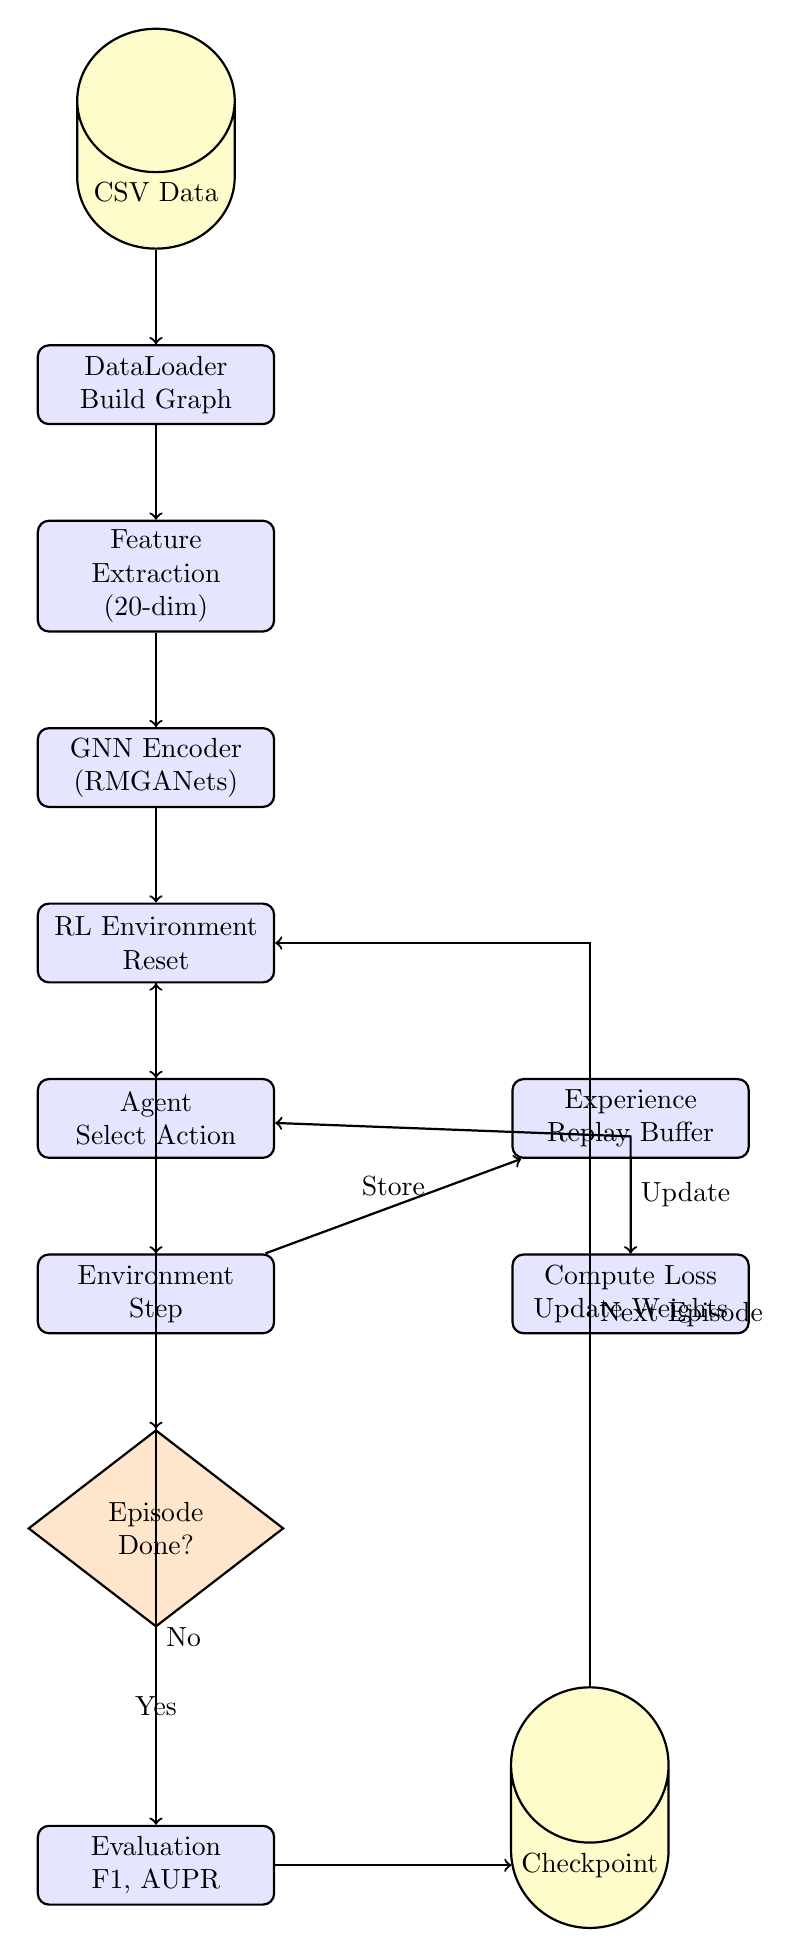
\begin{tikzpicture}[
    node distance=1.2cm,
    process/.style={rectangle, draw, thick, minimum width=3cm, minimum height=1cm, align=center, fill=blue!10, rounded corners},
    data/.style={cylinder, draw, thick, minimum width=2cm, minimum height=1cm, align=center, fill=yellow!20, shape border rotate=90},
    decision/.style={diamond, draw, thick, minimum width=2.5cm, minimum height=2.5cm, align=center, fill=orange!20, aspect=2},
    arrow/.style={->, thick}
]

    % Start
    \node[data] (csv) {CSV Data};

    % Data loading
    \node[process, below=of csv] (load) {DataLoader\\Build Graph};

    % Feature extraction
    \node[process, below=of load] (features) {Feature\\Extraction\\(20-dim)};

    % GNN encoding
    \node[process, below=of features] (gnn) {GNN Encoder\\(RMGANets)};

    % RL Environment
    \node[process, below=of gnn] (env) {RL Environment\\Reset};

    % Agent action
    \node[process, below=of env] (agent) {Agent\\Select Action};

    % Environment step
    \node[process, below=of agent] (step) {Environment\\Step};

    % Decision: Done?
    \node[decision, below=of step] (done) {Episode\\Done?};

    % Experience replay
    \node[process, right=3cm of agent] (replay) {Experience\\Replay Buffer};

    % Training
    \node[process, below=of replay] (train) {Compute Loss\\Update Weights};

    % Evaluation
    \node[process, below=2.5cm of done] (eval) {Evaluation\\F1, AUPR};

    % Checkpoint
    \node[data, right=3cm of eval] (checkpoint) {Checkpoint};

    % Arrows
    \draw[arrow] (csv) -- (load);
    \draw[arrow] (load) -- (features);
    \draw[arrow] (features) -- (gnn);
    \draw[arrow] (gnn) -- (env);
    \draw[arrow] (env) -- (agent);
    \draw[arrow] (agent) -- (step);
    \draw[arrow] (step) -- (done);
    \draw[arrow] (done) -- node[right] {No} ++(0,-1.5) -- (env);
    \draw[arrow] (done) -- node[above] {Yes} (eval);
    \draw[arrow] (step) -- node[above] {Store} (replay);
    \draw[arrow] (replay) -- (train);
    \draw[arrow] (train) -- node[right] {Update} ++(0,2) -- (agent);
    \draw[arrow] (eval) -- (checkpoint);
    \draw[arrow] (checkpoint) |- node[right, near start] {Next Episode} (env);

\end{tikzpicture}

\newpage

% ============================================================================
% DIAGRAM 5: Performance Comparison Bar Chart
% ============================================================================
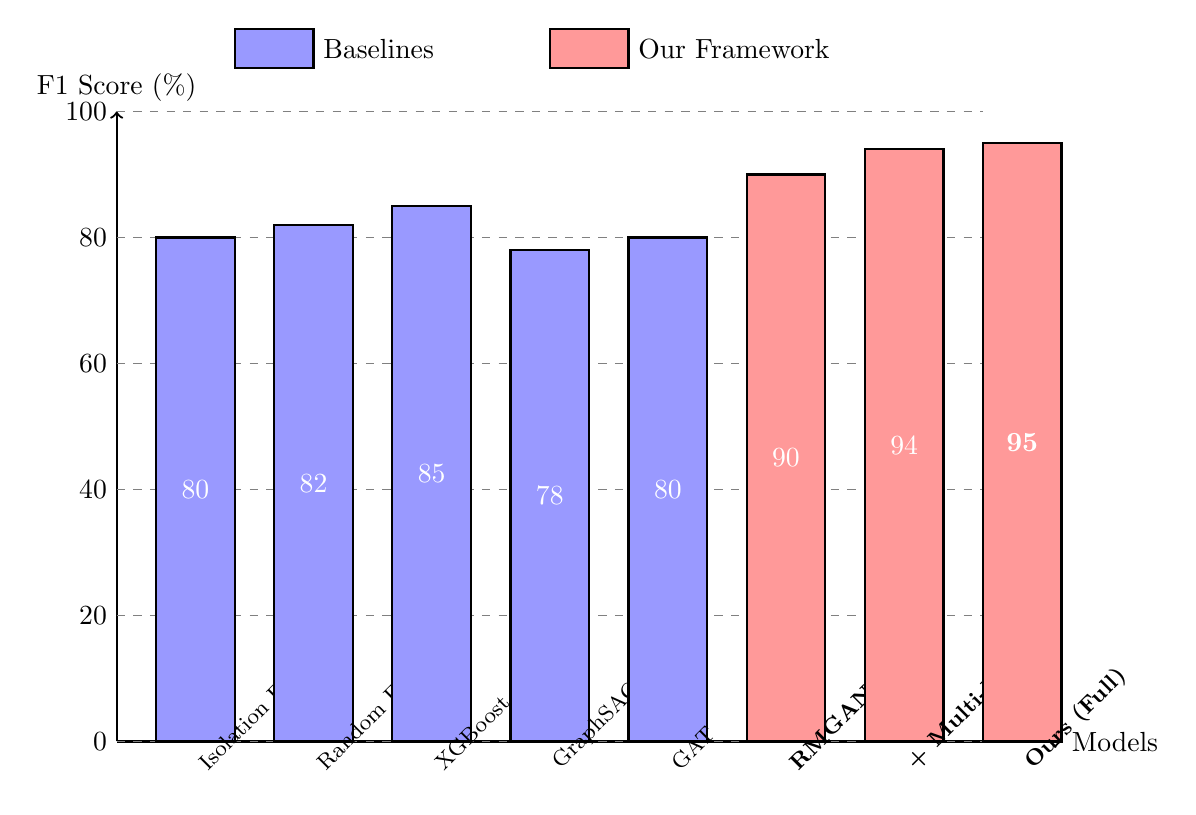
\begin{tikzpicture}[
    yscale=0.08,
    bar/.style={fill=blue!40, draw=black, thick},
    bar-ours/.style={fill=red!40, draw=black, thick},
    label/.style={font=\footnotesize, rotate=45, anchor=west}
]

    % Axes
    \draw[thick, ->] (0,0) -- (0,100) node[above] {F1 Score (\%)};
    \draw[thick, ->] (0,0) -- (12,0) node[right] {Models};

    % Grid
    \foreach \y in {0,20,40,60,80,100} {
        \draw[gray, dashed, thin] (0,\y) -- (11,\y);
        \node[left] at (0,\y) {\y};
    }

    % Bars
    \draw[bar] (0.5,0) rectangle (1.5,80) node[pos=0.5, white] {80};
    \node[label] at (1,-5) {Isolation Forest};

    \draw[bar] (2,0) rectangle (3,82) node[pos=0.5, white] {82};
    \node[label] at (2.5,-5) {Random Forest};

    \draw[bar] (3.5,0) rectangle (4.5,85) node[pos=0.5, white] {85};
    \node[label] at (4,-5) {XGBoost};

    \draw[bar] (5,0) rectangle (6,78) node[pos=0.5, white] {78};
    \node[label] at (5.5,-5) {GraphSAGE};

    \draw[bar] (6.5,0) rectangle (7.5,80) node[pos=0.5, white] {80};
    \node[label] at (7,-5) {GAT};

    \draw[bar-ours] (8,0) rectangle (9,90) node[pos=0.5, white] {90};
    \node[label] at (8.5,-5) {\textbf{RMGANets}};

    \draw[bar-ours] (9.5,0) rectangle (10.5,94) node[pos=0.5, white] {94};
    \node[label] at (10,-5) {\textbf{+ Multi-Branch}};

    \draw[bar-ours] (11,0) rectangle (12,95) node[pos=0.5, white] {\textbf{95}};
    \node[label] at (11.5,-5) {\textbf{Ours (Full)}};

    % Legend
    \node[bar, minimum width=1cm, minimum height=0.5cm] at (2,110) {};
    \node[right] at (2.5,110) {Baselines};
    \node[bar-ours, minimum width=1cm, minimum height=0.5cm] at (6,110) {};
    \node[right] at (6.5,110) {Our Framework};

\end{tikzpicture}

\end{document}
